% =====================================================================
%  A self-contained, step-by-step proof of the central theorem
%  ("Almost all Collatz orbits attain almost bounded values", Thm 1.3)
%  following the Idris2 formalization in this repository (TaoCollatz.*).
%
%  Margin notes tag every AXIOM (explicit hypothesis / analytic input)
%  and every LEMMA with its formal name; handwritten notes (rendered
%  from SVG via rsvg-convert, see make-handwritten.sh) appear in the
%  margins and inline.
%
%  Build:  ./make-handwritten.sh && pdflatex central-theorem.tex  (x2)
% =====================================================================
\documentclass[11pt]{article}

\usepackage[a4paper,left=22mm,right=52mm,top=24mm,bottom=26mm,
            marginparwidth=44mm,marginparsep=5mm]{geometry}
\usepackage{amsmath,amssymb,amsthm,mathtools}
\usepackage{xcolor}
\usepackage{graphicx}
\usepackage{marginnote}
\usepackage{enumitem}
\usepackage{seqsplit}
\usepackage{tikz}
\usetikzlibrary{arrows.meta,positioning}
\usepackage[colorlinks=true,linkcolor=blue!55!black,citecolor=blue!55!black,
            urlcolor=blue!55!black]{hyperref}

\renewcommand{\marginfont}{\footnotesize}

% ---- colours -------------------------------------------------------
\definecolor{axcol}{RGB}{160,24,24}     % axioms  (red)
\definecolor{lemcol}{RGB}{18,48,122}    % lemmas  (blue)
\definecolor{defcol}{RGB}{28,107,42}    % defs    (green)
\definecolor{inkblue}{RGB}{18,48,122}

% ---- margin tags ---------------------------------------------------
% #1 colour  #2 kind label  #3 formal name  #4 optional note
\newcommand{\margtag}[4]{%
  \marginnote{\raggedright\scriptsize
    \colorbox{#1}{\textcolor{white}{\bfseries #2}}\\[3pt]
    {\ttfamily\textcolor{#1}{\seqsplit{#3}}}%
    \ifx\relax#4\relax\else\\[2pt]\textit{#4}\fi}}
\newcommand{\axmarg}[2][\relax]{\margtag{axcol}{AXIOM}{#2}{#1}}
\newcommand{\lemmarg}[2][\relax]{\margtag{lemcol}{LEMMA}{#2}{#1}}
\newcommand{\defmarg}[2][\relax]{\margtag{defcol}{DEF}{#2}{#1}}

% ---- handwritten margin / inline notes -----------------------------
\newcommand{\hwmarg}[2][42mm]{\marginnote{\includegraphics[width=#1]{handwritten/#2}}}
\newcommand{\hwinline}[2][32mm]{%
  \raisebox{-2pt}{\includegraphics[width=#1]{handwritten/#2}}}

% ---- theorem-like environments ------------------------------------
\theoremstyle{definition}
\newtheorem{defn}{Definition}[section]
\theoremstyle{plain}
\newtheorem{thm}{Theorem}[section]
\newtheorem{lem}[thm]{Lemma}
\newtheorem{prop}[thm]{Proposition}
\newtheorem{cor}[thm]{Corollary}
\theoremstyle{remark}
\newtheorem{ax}{Axiom / Hypothesis}
\newtheorem*{rem}{Remark}

% ---- notation ------------------------------------------------------
\newcommand{\N}{\mathbb{N}}
\newcommand{\Col}{\operatorname{\mathsf{Col}}}
\newcommand{\Syr}{\operatorname{\mathsf{Syr}}}
\newcommand{\odd}{\operatorname{\mathsf{odd}}}
\newcommand{\oddPart}{\operatorname{\mathsf{oddPart}}}
\newcommand{\half}{\operatorname{\mathsf{half}}}
\newcommand{\iter}[1]{\mathrm{iter}_{#1}}
\newcommand{\Pos}{\mathsf{Pos}}
\newcommand{\OddPos}{\mathsf{OddPos}}
\newcommand{\dropT}{\operatorname{\mathsf{dropTime}}}
\newcommand{\ColBelow}{\mathsf{ColBelow}}
\newcommand{\SyrBelow}{\mathsf{SyrBelow}}
\newcommand{\AlAll}{\mathsf{AlmostAll}}
\newcommand{\eqdef}{\vcentcolon=}

\begin{document}

% ===================================================================
\begin{center}
  {\LARGE\bfseries A Self-Contained Proof of the Central Theorem}\\[4pt]
  {\large Almost all Collatz orbits attain almost bounded values (Theorem 1.3)}\\[10pt]
  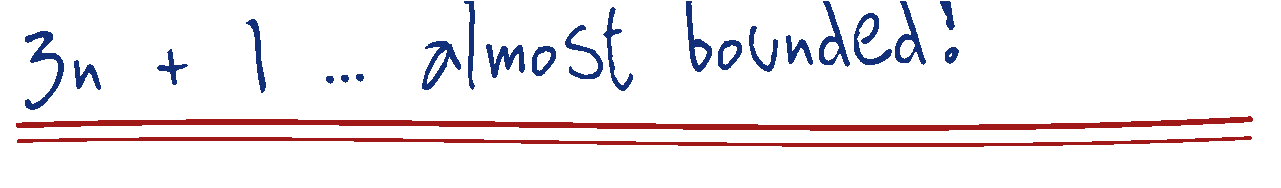
\includegraphics[width=0.62\linewidth]{handwritten/hw_title}\\[8pt]
  {\normalsize A step-by-step account tracking the Idris2 formalization
   \texttt{TaoCollatz.*}}\\[2pt]
  {\small\today}
\end{center}

\vspace{4pt}
\hrule
\vspace{10pt}

% ===================================================================
\section{Overview}\label{sec:overview}

This note proves, from first principles and in a self-contained way, the
central theorem of Terence Tao's paper \emph{Almost all Collatz orbits attain
almost bounded values} (Theorem~1.3), exactly as it is formalized in this
repository.  Every definition, axiom, and lemma below carries a margin tag with
the name of the corresponding Idris2 declaration, so the document doubles as a
readable transcript of the mechanized proof.

\hwmarg{hw_fourarrows}
The proof is deliberately \emph{modular}: the whole argument is a single
composition of four independent one-step reductions, each carrying one milestone
of the paper to the next,
\[
  \underbrace{\text{analytic input}}_{\text{Props 1.9, 7.8}}
  \;\Longrightarrow\;
  \underbrace{\text{first-passage stabilisation}}_{\text{Prop 1.11}}
  \;\Longrightarrow\;
  \underbrace{\text{Thm 3.1}}_{\text{quantitative}}
  \;\Longrightarrow\;
  \underbrace{\text{Thm 1.6}}_{\text{Syracuse}}
  \;\Longrightarrow\;
  \underbrace{\text{Thm 1.3}}_{\text{Collatz}} .
\]
Two ingredients are genuinely irreducible and are therefore taken as explicit
hypotheses (never fabricated): a \emph{growth-compatible odd-threshold system}
and the \emph{deep analytic first-passage input} (Propositions 1.9 and 7.8).
Everything else --- in particular the dynamical heart of the reduction, the
identification of the Syracuse map with the odd part of the Collatz map
(\S\ref{sec:oddpart}) --- is proved outright.

\begin{center}
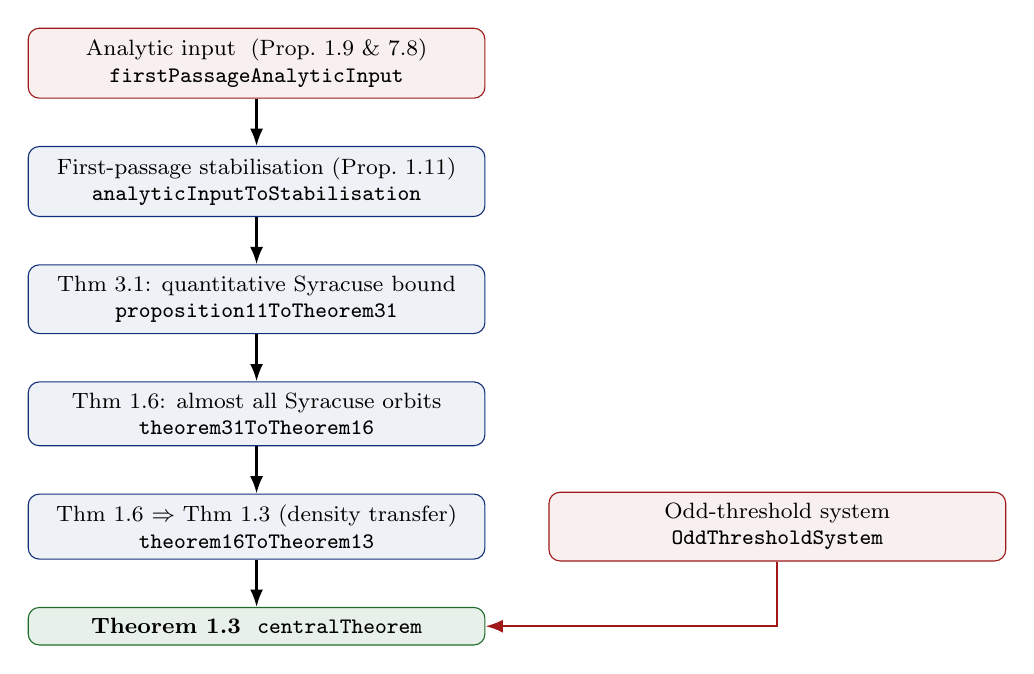
\begin{tikzpicture}[
    node distance=6mm and 0mm,
    box/.style={draw,rounded corners,align=center,inner sep=4pt,
                font=\footnotesize,minimum width=58mm},
    ax/.style={box,draw=axcol,fill=axcol!7},
    lm/.style={box,draw=lemcol,fill=lemcol!7},
    goal/.style={box,draw=defcol,fill=defcol!10,font=\footnotesize\bfseries},
    ar/.style={-{Latex[length=2.2mm]},thick}]
  \node[ax] (ana) {Analytic input \;(Prop.\ 1.9 \& 7.8)\\\texttt{firstPassageAnalyticInput}};
  \node[lm,below=of ana] (stab) {First-passage stabilisation (Prop.\ 1.11)\\\texttt{analyticInputToStabilisation}};
  \node[lm,below=of stab] (t31) {Thm 3.1: quantitative Syracuse bound\\\texttt{proposition11ToTheorem31}};
  \node[lm,below=of t31] (t16) {Thm 1.6: almost all Syracuse orbits\\\texttt{theorem31ToTheorem16}};
  \node[lm,below=of t16] (t13) {Thm 1.6 $\Rightarrow$ Thm 1.3 (density transfer)\\\texttt{theorem16ToTheorem13}};
  \node[goal,below=of t13] (goal) {\textbf{Theorem 1.3} \;\texttt{centralTheorem}};
  \node[ax,right=8mm of t13] (sys) {Odd-threshold system\\\texttt{OddThresholdSystem}};
  \draw[ar] (ana)--(stab); \draw[ar] (stab)--(t31); \draw[ar] (t31)--(t16);
  \draw[ar] (t16)--(t13); \draw[ar] (t13)--(goal);
  \draw[ar,axcol] (sys.south) |- (goal.east);
\end{tikzpicture}
\end{center}

% ===================================================================
\section{The dynamical objects}\label{sec:objects}

We work throughout with the unary natural numbers $\N=\{0,1,2,\dots\}$ and the
iteration operator
\[
  \iter{0} f\,x = x, \qquad \iter{k+1} f\,x = \iter{k} f\,(f\,x),
\]
which satisfies the shift law $\iter{m+n} f\,x = \iter{n} f\,(\iter{m} f\,x)$.
\defmarg[iterate a map; \texttt{iterPlus}]{Core.iter}
We order $\N$ by the inductive relation $\le$ (\texttt{Leq}), which is reflexive
and transitive.

\begin{defn}[Carriers]\label{def:carriers}
\defmarg{Dynamics.Pos, OddPos}
$\Pos$ is a wrapper around a single natural number $n$ (its \emph{value}), and
$\OddPos$ likewise; their \emph{heights} are $\mathsf{posSize}(n)=n$ and
$\mathsf{oddSize}(n)=n$.  The paper's genuine domains --- the positive integers
and the odd positive integers --- are recovered by the predicates
$\mathsf{PaperPositive}$ and $\mathsf{PaperOddPositive}$.
\end{defn}

\begin{defn}[Halving and the odd factor]\label{def:oddfactor}
\defmarg[strip factors of $2$; \texttt{oddFactorFuel}]{Dynamics.half, oddFactor}
Let $\half(0)=0$, $\half(1)=0$, $\half(n+2)=\half(n)+1$, so that
$\half(n)=\lfloor n/2\rfloor$.  The \emph{odd factor} $\odd(n)$ is obtained by
repeatedly halving $n$ while it is even; formally, with fuel $f$,
\[
  \odd_f(n) \eqdef
  \begin{cases}
    n & f=0,\\
    \odd_{f-1}(\half n) & f>0,\ n\text{ even},\\
    n & f>0,\ n\text{ odd},
  \end{cases}
  \qquad \odd(n)\eqdef \odd_n(n).
\]
The \emph{drop time} $\dropT(n)$ counts how many halvings this takes.
\end{defn}

\begin{defn}[The Collatz and Syracuse maps]\label{def:maps}
\defmarg[$3n{+}1$ dynamics; \texttt{Col, Syr}]{Dynamics.Col, Syr}
On $\Pos$ the \emph{Collatz map} is
\[
  \Col(n) \eqdef
  \begin{cases}
    \half(n) & n\text{ even},\\
    3n+1 & n\text{ odd},
  \end{cases}
\]
and on $\OddPos$ the \emph{Syracuse map} is $\Syr(n)\eqdef \odd(3n+1)$.
The \emph{odd part} map $\oddPart\colon\Pos\to\OddPos$ sends $n\mapsto\odd(n)$.
\end{defn}

\hwmarg{hw_check}
As numeric sanity checks (all verified by \texttt{Refl} in the formalization):
$\Col(3)=10$, $\Col^{2}(3)=5$, $\Syr(7)=11$, $\oddPart(12)=3$, and
$\dropT(12)=2$.

% ===================================================================
\section{Convergence, growth, and ``almost all''}\label{sec:framework}

\begin{defn}[Eventually below a bound]\label{def:below}
\defmarg[reach height $\le b$; \texttt{EventuallyBelow}]{Core.EventuallyBelow}
For a system $(A,\mathrm{step},\mathrm{height})$, a point $x$ is
\emph{eventually below} $b$ if there is a time $t$ with
$\mathrm{height}\bigl(\iter{t}\mathrm{step}\,x\bigr)\le b$.  Specialising to the
two maps,
\[
  \ColBelow(n,b)\eqdef \text{$n$ eventually below $b$ under }\Col,\qquad
  \SyrBelow(n,b)\eqdef \text{$n$ eventually below $b$ under }\Syr.
\]
If $x$ is eventually below $b$ and $b\le b'$, then $x$ is eventually below $b'$
(\texttt{eventuallyMonotoneBound}), by transitivity of $\le$.
\end{defn}

\begin{defn}[Tending to infinity]\label{def:growth}
\defmarg[$f(x)\to\infty$; \texttt{TendsToInfinityOn}]{Large.TendsToInfinityOn}
A function $f$ on a carrier with height \emph{tends to infinity} if for every
target $t$ there is a height threshold beyond which $f\ge t$.  The identity
heights $\mathsf{posSize}$ and $\mathsf{oddSize}$ tend to infinity, growth is
monotone under $f\le g$ (\texttt{growthMonotone}), and $f\to\infty$ implies
$\mathrm{pred}\circ f\to\infty$ (\texttt{growthPred}).
\end{defn}

\begin{defn}[Logarithmically small / almost all]\label{def:almostall}
\defmarg[vanishing exceptional set; \texttt{ExceptionalControl}]{Large.AlmostAllOn}
A predicate $q$ holds for \emph{almost all} $x$ (written $\AlAll_A q$) if there is a
``controlled'' sub-predicate $c$ such that
\begin{enumerate}[label=(\alph*),nosep]
  \item $c(x)\Rightarrow q(x)$ for all $x$ \hfill(\texttt{controlledImplies}),
  \item the set where $c$ fails is \emph{logarithmically small}: it carries an
        error bound $E\colon\N\to\N$ with $E(N)\to 0$ as the cutoff
        $N\to\infty$ \hfill(\texttt{LogarithmicSmallness}, \texttt{VanishesAtInfinity}).
\end{enumerate}
\end{defn}

\hwmarg{hw_almostall}
\noindent At the resolution of this development the analytic magnitude of the
exceptional set is represented structurally (a vanishing error bound together
with a certificate); the two closure lemmas we need are proved in full:

\begin{lem}[Monotonicity of ``almost all'']\label{lem:aamap}
\lemmarg[push a pointwise implication forward]{Large.almostAllMap}
If $\AlAll_A p$ holds and $p(x)\Rightarrow q(x)$ for every $x$, then $\AlAll_A q$.
\end{lem}
\begin{proof}
Keep the same controlled predicate $c$ and the same (vanishing) error bound;
only the final implication changes, composing $c(x)\Rightarrow p(x)$ with
$p(x)\Rightarrow q(x)$ to get $c(x)\Rightarrow q(x)$.
\end{proof}

\begin{lem}[Pullback of ``almost all'']\label{lem:aapull}
\lemmarg[transport along a map; \texttt{almostAllPullback}]{Large.controlPullback}
Let $\varphi\colon A\to B$ and let $p$ be a predicate on $B$ with $\AlAll_B p$.
Then $\AlAll_A\bigl(x\mapsto p(\varphi x)\bigr)$.
\end{lem}
\begin{proof}
Take the controlled predicate $x\mapsto c(\varphi x)$ and the same error bound;
$c(\varphi x)\Rightarrow p(\varphi x)$ is inherited pointwise.
\end{proof}

\begin{lem}[Certified control]\label{lem:aacert}
\lemmarg[a proof of $p$ gives ``almost all $p$'']{Large.controlByProperty}
If a predicate $p$ holds for all $x$ (witnessed by any certificate), then
$\AlAll_A p$, with the identically-zero error bound.
\end{lem}

% ===================================================================
\section{The statements}\label{sec:statements}

\begin{defn}[The three milestones]\label{def:milestones}
\defmarg[Thm 1.3 / 1.6 / 3.1]{Large.Theorem13, Dependencies}
\begin{description}[leftmargin=0pt,itemsep=3pt,style=nextline]
  \item[Thm 1.3 \normalfont(\texttt{Theorem13}).]
    For every $f\to\infty$ on $\Pos$,\;
    $\AlAll_{\Pos}\bigl(n\mapsto \ColBelow(n,f(n))\bigr)$.
  \item[Thm 1.6 \normalfont(\texttt{Theorem16}).]
    For every $f\to\infty$ on $\OddPos$,\;
    $\AlAll_{\OddPos}\bigl(n\mapsto \SyrBelow(n,f(n))\bigr)$.
  \item[Thm 3.1 \normalfont(\texttt{QuantitativeSyracuseBound}).]
    For every $f\to\infty$ on $\OddPos$,\;
    $\AlAll_{\OddPos}\bigl(n\mapsto \SyrBelow(n,f(n))\bigr)$.
\end{description}
Theorems 1.6 and 3.1 have the same shape here: Thm 3.1 is the quantitative
route by which Thm 1.6 is obtained.  The strict and paper-domain reformulations
of Thm 1.3 (\texttt{Theorem13Strict}, \texttt{Theorem13PaperDomain}) replace the
bound $f(n)$ by $f(n)-1$ and restrict to genuine positive integers.
\end{defn}

% ===================================================================
\section{The two irreducible inputs (axioms)}\label{sec:axioms}

The whole theorem rests on exactly two ingredients that are \emph{not}
constructible here and are taken as honest hypotheses.

\hwmarg{hw_assume}
\begin{ax}[Growth-compatible odd-threshold system]\label{ax:sys}
\axmarg[not a computable function of $f$]{PaperInterfaces.OddThresholdSystem}
There is an assignment sending each height function $f$ on $\Pos$ to a threshold
function $\theta_f$ on $\OddPos$ such that
\begin{enumerate}[label=(\roman*),nosep]
  \item \emph{(growth)} if $f\to\infty$ then $\theta_f\to\infty$
        \hfill(\texttt{oddThresholdGrows});
  \item \emph{(compatibility)} $\theta_f(\oddPart\,n)\le f(n)$ for every
        $n\in\Pos$ \hfill(\texttt{thresholdCompatibility}).
\end{enumerate}
\end{ax}

\begin{rem}
\hwmarg{hw_threshold}
This is genuinely not a total computable function of $f$ alone: the zero
threshold satisfies compatibility but fails growth, while a growing choice needs
an infimum over each odd fibre $\oddPart^{-1}(m)$ (equivalently, the growth
witness of $f$).  It is classically inhabited; the formalization threads it in
as a hypothesis rather than fabricating it, so no soundness is lost.
\end{rem}

\begin{ax}[Deep first-passage analytic input]\label{ax:analytic}
\axmarg[Props 1.9 \& 7.8]{Dependencies.firstPassageAnalyticInput}
We are given the pair
$\bigl(\textsf{ValuationDistribution},\ \textsf{StabilityPrinciple}\bigr)$
consisting of
\begin{enumerate}[label=(\roman*),nosep]
  \item the \emph{$2$-adic valuation tail estimate} for the Syracuse map
        (Proposition~1.9), and
  \item the \emph{renewal / stability principle} producing a first-passage
        stability estimate from the valuation distribution
        (Proposition~7.8, via the chain $7.8\!\Rightarrow\!7.3\!\Rightarrow\!
        7.1\!\Rightarrow\!1.17\!\Rightarrow\!1.14$).
\end{enumerate}
\end{ax}

\hwmarg{hw_deep}
\begin{rem}
These are the genuinely hard analytic theorems of the paper.  In this
development their payload types are opaque placeholders, honestly inhabited (no
\texttt{believe\_me}); they are exactly the leaves that a full analytic
formalization would replace with real estimates.  The complete paper skeleton
$7.8\Rightarrow\cdots\Rightarrow1.14$ is recorded in
\texttt{TaoCollatz.PaperStructure}.
\end{rem}

% ===================================================================
\section{The dynamical heart: Syracuse is the odd part of Collatz}
\label{sec:oddpart}

\hwmarg{hw_syracuse}
This section proves the one substantial dynamical fact of the reduction: that a
Syracuse orbit is exactly what a Collatz orbit does once the powers of $2$ are
stripped away.  Everything here is proved outright.

\begin{lem}[Arithmetic of halving]\label{lem:half}
\lemmarg[\texttt{halfLe, halfLtSelf, halfNonZero}]{OddPart.half*}
For all $n$: $\half(n)\le n$; if $n\ne 0$ then $\half(n)<n$; and if $n$ is even
and $n\ne 0$ then $\half(n)\ne 0$.
\end{lem}
\begin{proof}
Each is a two-step induction on $n$ (base cases $n=0,1$; step $n\mapsto n+2$
uses the recursion $\half(n+2)=\half(n)+1$).
\end{proof}

\begin{lem}[The odd factor is odd]\label{lem:oddodd}
\lemmarg[with enough fuel; \texttt{oddFactorOdd}]{OddPart.oddFactorOdd}
If $n\ne 0$ then $\odd(n)$ is odd.
\end{lem}
\begin{proof}
Induct on the fuel.  If $n$ is odd the halving loop stops immediately and
returns $n$.  If $n$ is even and nonzero, then by Lemma~\ref{lem:half}
$\half(n)$ is nonzero and strictly smaller, so one unit of fuel is consumed and
the claim follows for $\odd(\half n)=\odd(n)$ by induction.  Starting with
$n$ units of fuel is always enough because each step strictly decreases the
value (\texttt{leqHalfFuel}).
\end{proof}

\begin{lem}[A Collatz step on an odd number]\label{lem:colodd}
\lemmarg[$\Col(m)=3m{+}1$ for odd $m$]{OddPart.colOdd}
If $m$ is odd then $\Col(m)=3m+1$.
\end{lem}
\begin{proof}
Immediate from Definition~\ref{def:maps} once the even-test evaluates to false.
\end{proof}

\begin{lem}[Normalisation reaches the odd factor]\label{lem:normalize}
\lemmarg[drop the even part; \texttt{oddPartDropTimeNormalizesValue}]{Dynamics/OddPart.normalizeToPos}
For every $n$, iterating $\Col$ exactly $\dropT(n)$ times from $n$ lands on the
value $\odd(n)$:
$\;\iter{\dropT(n)}\Col\,n = \odd(n)$.
\end{lem}
\begin{proof}
Induct on the fuel used by $\dropT$ and $\odd$ in lock-step
(\texttt{oddFactorFuelColNormalize}).  While $n$ is even, one Collatz step is a
halving, matching one halving inside $\odd$; when $n$ becomes odd both stop.
\end{proof}

\begin{lem}[One Syracuse step, realised inside the Collatz orbit]\label{lem:realizestep}
\lemmarg[glue: $3m{+}1$ then normalise]{OddPart.syrRealizeStep}
Let $m$ be odd and suppose the Collatz orbit realises the height of the
$k$-th Syracuse iterate started from $\odd(3m+1)$.  Then it also realises the
height of the $(k{+}1)$-st Syracuse iterate started from $m$, after
$1+\dropT(3m+1)+s'$ Collatz steps.
\end{lem}
\begin{proof}
By Lemma~\ref{lem:colodd} the first Collatz step sends $m$ to $3m+1$; by
Lemma~\ref{lem:normalize} the next $\dropT(3m+1)$ steps normalise $3m+1$ to
$\odd(3m+1)=\Syr(m)$; the shift law $\iter{a+b}=\iter{b}\circ\iter{a}$
then splices the assumed realisation of the remaining $k$ Syracuse steps.
\end{proof}

\begin{lem}[Exact Collatz/Syracuse correspondence]\label{lem:realize}
\lemmarg[$\forall t\ \exists s$; \texttt{syrRealize}]{OddPart.syrRealize}
For every odd $m$ and every $t$ there is a Collatz time $s$ with
\[
  \iter{s}\Col\,m \;=\; \iter{t}\Syr\,m .
\]
\end{lem}
\begin{proof}
Induct on $t$.  For $t=0$ take $s=0$.  For $t=k+1$, apply the induction
hypothesis to the odd number $\odd(3m+1)$ (odd by Lemma~\ref{lem:oddodd}) to get
$s'$, then Lemma~\ref{lem:realizestep} yields
$s=1+\dropT(3m+1)+s'$.
\end{proof}

\begin{lem}[Height domination]\label{lem:heightbound}
\lemmarg[for every $\Pos$; \texttt{oddPartHeightBoundAt}]{OddPart.oddPartHeightBoundAt}
For every $x\in\Pos$ and every Syracuse time $t$ there is a Collatz time $s$
with
\[
  \mathsf{posSize}\bigl(\iter{s}\Col\,x\bigr)\;\le\;
  \mathsf{oddSize}\bigl(\iter{t}\Syr\,(\oddPart\,x)\bigr).
\]
\end{lem}
\begin{proof}
If $x=0$ take $s=0$ (heights are $0$).  Otherwise write $x=k+1$; normalise to
$\odd(k+1)$ in $\dropT(k+1)$ steps (Lemma~\ref{lem:normalize}) and then invoke
the correspondence of Lemma~\ref{lem:realize} for the odd value $\odd(k+1)$.
Combining the two gives an \emph{equality} of heights, hence in particular the
required $\le$ (\texttt{oddPartHeightEqPos}, \texttt{leqOfEq}).
\end{proof}

\begin{prop}[Odd-part orbit simulation]\label{prop:sim}
\lemmarg[the whole point; \texttt{provenOddPartOrbitSimulation}]{OddPart.provenOddPartOrbitSimulation}
The map $\oddPart\colon\Pos\to\OddPos$ is a height-dominating semiconjugacy from
$(\Pos,\Col)$ to $(\OddPos,\Syr)$: there is a function
$(x,t)\mapsto s(x,t)$ with
$\mathsf{posSize}(\iter{s(x,t)}\Col\,x)\le
 \mathsf{oddSize}(\iter{t}\Syr\,(\oddPart\,x))$
for all $x,t$.  In the terminology of \S\ref{sec:framework} this is an
\texttt{OrbitSimulation}.
\end{prop}
\begin{proof}
Take $s(x,t)$ and its bound directly from Lemma~\ref{lem:heightbound}.
\end{proof}

\begin{cor}[Transfer of ``eventually below'']\label{cor:transfer}
\lemmarg[$\SyrBelow\Rightarrow\ColBelow$]{Core.simulationTransfersEventuallyBelow}
For every $x\in\Pos$ and bound $b$,
$\;\SyrBelow(\oddPart\,x,\,b)\Rightarrow \ColBelow(x,b)$.
\end{cor}
\begin{proof}
If the Syracuse orbit of $\oddPart\,x$ is below $b$ at time $t$, then by
Proposition~\ref{prop:sim} the Collatz orbit of $x$ is below the same value ---
hence below $b$ --- at time $s(x,t)$ (transitivity of $\le$).
\end{proof}

\hwmarg{hw_nobelieveme}
\begin{rem}
Corollary~\ref{cor:transfer} is the only place where the concrete Collatz/
Syracuse dynamics enter, and it is proved with no axioms and no
\texttt{believe\_me}.  It is also an instance of a reusable \emph{simulation
algebra}: orbit simulations form a category with identity
(\texttt{orbitSimulationId}) and composition (\texttt{orbitSimulationCompose}).
\end{rem}

% ===================================================================
\section{The density transfer: Thm 1.6 $\Rightarrow$ Thm 1.3}\label{sec:transfer}

\begin{lem}[Threshold weakening]\label{lem:weaken}
\lemmarg[compatibility relaxes the bound]{Dependencies.oddPartThresholdToReachability}
Fix an odd-threshold system (Axiom~\ref{ax:sys}) with thresholds $\theta$.
For every $f$ and $n\in\Pos$,
\[
  \SyrBelow\bigl(\oddPart\,n,\ \theta_f(\oddPart\,n)\bigr)\ \Longrightarrow\
  \SyrBelow\bigl(\oddPart\,n,\ f(n)\bigr).
\]
\end{lem}
\begin{proof}
By compatibility $\theta_f(\oddPart\,n)\le f(n)$, so this is monotonicity of
$\SyrBelow$ in the bound (Definition~\ref{def:below}).
\end{proof}

\begin{lem}[Density lift]\label{lem:lift}
\lemmarg[pull odd control back to $\Pos$]{Dependencies.oddPartDensityLift}
With the same system, if almost all odd numbers $m$ satisfy
$\SyrBelow(m,\theta_f(m))$, then almost all $n\in\Pos$ satisfy
$\SyrBelow(\oddPart\,n, f(n))$.
\end{lem}
\begin{proof}
Pull the odd-side statement back along $\oddPart$ (Lemma~\ref{lem:aapull}) to get
almost all $n$ with $\SyrBelow(\oddPart\,n,\theta_f(\oddPart\,n))$, then apply
Lemma~\ref{lem:weaken} pointwise via monotonicity (Lemma~\ref{lem:aamap}).
\end{proof}

\begin{thm}[Syracuse $\Rightarrow$ Collatz density transfer]\label{thm:t16to13}
\lemmarg[Thm 1.6 $\Rightarrow$ Thm 1.3]{Dependencies.theorem16ToTheorem13}
An odd-threshold system (Axiom~\ref{ax:sys}) turns Theorem~1.6 into
Theorem~1.3.
\end{thm}
\begin{proof}
Let $f\to\infty$ on $\Pos$.  By growth of the system, $\theta_f\to\infty$ on
$\OddPos$, so Theorem~1.6 applied to $\theta_f$ gives that almost all odd $m$
satisfy $\SyrBelow(m,\theta_f(m))$.  Lemma~\ref{lem:lift} lifts this to: almost
all $n\in\Pos$ satisfy $\SyrBelow(\oddPart\,n,f(n))$.  Finally
Corollary~\ref{cor:transfer} converts each such Syracuse statement into
$\ColBelow(n,f(n))$, pointwise, and Lemma~\ref{lem:aamap} pushes it through the
``almost all''.  This is exactly Theorem~1.3.
\end{proof}

% ===================================================================
\section{The analytic reductions: input $\Rightarrow$ Thm 3.1 $\Rightarrow$ Thm 1.6}
\label{sec:analytic}

\begin{lem}[First-passage stabilisation, Prop.\ 1.11]\label{lem:stab}
\lemmarg[assemble the two estimates]{Dependencies.analyticInputToStabilisation}
The analytic input (Axiom~\ref{ax:analytic}) yields a \emph{stabilisation of
first passage}: the pair of a tail estimate and a stability estimate, the latter
produced by feeding the valuation distribution to the stability principle.
\end{lem}

\begin{lem}[Prop.\ 1.11 $\Rightarrow$ Theorem 3.1]\label{lem:t31}
\lemmarg[iterate to a uniform bound]{Dependencies.proposition11ToTheorem31}
A stabilisation of first passage yields the quantitative Syracuse bound: for
each $f\to\infty$ on $\OddPos$, almost all odd numbers reach below $f$.
\end{lem}
\begin{proof}
The stabilisation certifies, for each growing $f$, the control predicate
$\SyrBelow(\cdot,f(\cdot))$ with a vanishing exceptional error bound; this is
precisely $\AlAll_{\OddPos}(m\mapsto\SyrBelow(m,f(m)))$ by
Lemma~\ref{lem:aacert} (\texttt{firstPassageToQuantitativeBound}).
\end{proof}

\begin{lem}[Theorem 3.1 $\Rightarrow$ Theorem 1.6]\label{lem:t16}
\lemmarg[same statement]{Dependencies.theorem31ToTheorem16}
The quantitative Syracuse bound is Theorem~1.6.
\end{lem}
\begin{proof}
The two statements coincide (Definition~\ref{def:milestones}).
\end{proof}

% ===================================================================
\section{Assembly of the central theorem}\label{sec:assembly}

\hwmarg{hw_fourarrows}
Nothing remains but to chain the reductions of the previous sections together.

\begin{thm}[Central theorem, Theorem 1.3]\label{thm:central}
\lemmarg[the goal]{Dependencies.centralTheorem}
Given a growth-compatible odd-threshold system (Axiom~\ref{ax:sys}) and the deep
first-passage analytic input (Axiom~\ref{ax:analytic}), almost all Collatz
orbits attain almost bounded values:
\[
  \forall f\to\infty\ \text{on }\Pos,\qquad
  \AlAll_{\Pos}\bigl(n\mapsto \ColBelow(n,f(n))\bigr).
\]
\end{thm}
\begin{proof}
Compose the four reductions established above:
\[
  \underbrace{\text{Lem.}~\ref{lem:stab}}_{\text{input}\,\Rightarrow\,\text{Prop 1.11}}
  \ \longrightarrow\
  \underbrace{\text{Lem.}~\ref{lem:t31}}_{\Rightarrow\,\text{Thm 3.1}}
  \ \longrightarrow\
  \underbrace{\text{Lem.}~\ref{lem:t16}}_{\Rightarrow\,\text{Thm 1.6}}
  \ \longrightarrow\
  \underbrace{\text{Thm.}~\ref{thm:t16to13}}_{\Rightarrow\,\text{Thm 1.3}} .
\]
Feeding the analytic input of Axiom~\ref{ax:analytic} through
Lemmas~\ref{lem:stab}--\ref{lem:t16} produces Theorem~1.6; the odd-threshold
system of Axiom~\ref{ax:sys} then turns it into Theorem~1.3 by
Theorem~\ref{thm:t16to13}.  This composite is precisely
\texttt{centralTheoremFromInputs}, and it is definitionally equal to the
\texttt{DualProof}-based \texttt{centralTheorem}
(\texttt{centralTheoremUnifiedAgrees}, proved by \texttt{Refl}).
\end{proof}
\hfill\hwinline[30mm]{hw_qed}

\begin{cor}[Reformulations]\label{cor:reform}
\lemmarg[strict / paper-domain]{Dependencies.centralTheoremStrict, PaperDomain}
Under the same hypotheses, the strict-bound form (bound $f(n)-1$) and the
paper-domain form (restricted to genuine positive integers) also hold,
obtained from Theorem~\ref{thm:central} by the packaging adapters
\texttt{theorem13StrictFromNonStrict} and
\texttt{theorem13PaperDomainFromStrict}.
\end{cor}

% ===================================================================
\section{What is proved, and what is assumed}\label{sec:status}

\hwmarg{hw_nobelieveme}
The development contains \textbf{no} \texttt{believe\_me}, \textbf{no} axioms in
the Idris sense, and \textbf{no} holes; every definition is total.  Concretely:

\begin{itemize}[nosep,leftmargin=1.4em]
  \item \textbf{Proved outright.} The concrete dynamics ($\Col,\Syr,\odd,\dropT$)
        and their numeric checks; the entire odd-part correspondence of
        \S\ref{sec:oddpart} (Lemmas~\ref{lem:half}--\ref{cor:transfer}); the
        ``almost all'' closure lemmas of \S\ref{sec:framework}; and the full
        reduction plumbing of \S\S\ref{sec:transfer}--\ref{sec:assembly}.
  \item \textbf{Explicit hypotheses (Axioms~\ref{ax:sys},~\ref{ax:analytic}).}
        The growth-compatible odd-threshold system, and the deep analytic
        first-passage input (Propositions 1.9 and 7.8).  These are the leaves a
        complete analytic formalization would discharge; here they are honest
        placeholders, not fabricated proofs.
\end{itemize}

Thus the honest reading of the result is the \emph{conditional}
\[
  \texttt{centralTheorem} : \textsf{OddThresholdSystem} \longrightarrow
  \textsf{Theorem13},
\]
with the analytic input supplied internally as a structural placeholder.  The
mathematical content that is genuinely mechanized --- above all the
identification of the Syracuse map with the odd part of the Collatz map --- is
exactly the reduction structure of Tao's argument.

\vspace{6pt}
\begin{center}\small\itshape
Every margin tag names the Idris2 declaration it summarises; see
\texttt{TaoCollatz/} for the machine-checked source.
\end{center}

\end{document}
